\chapter{Transfer Learning}
\label{ch-transfer}

Historically,
the term Transfer Learning (TL)
has been used in AI mostly by Artificial Neural Net (ANN)
proponents (see the Wikipedia article on TL,
 Ref.\cite{wiki-TL}).
Recently, however,
 a theory of causal TL
has begun to emerge
(see Chapter \ref{ch-transfer-causal}).

TL in AI is a
fairly wide topic that 
is somewhat ambiguously defined.
Some subjects that can be lumped
under the heading of TL in AI are:
\begin{itemize}
\item data fusion/combining models
\item model generalization
\item transportability of 
causal knowledge, external validity
(see Chapter \ref{ch-transfer-causal})
\end{itemize}


Most AI researchers
will agree that it is highly desirable 
to have TL in AI, because the human 
brain obviously does  plenty of TL
to great advantage.
Although reams of papers 
have been written about the subject of TL in AI,
a systematic theory of TL in AI
that is universally accepted and popular
remains elusive. The current
theory of \ul{TL for ANN} looks to me 
like a grab bag
of
 heuristic approaches
that are fragile, meaning they
can be easily spoofed.
The theory of \ul{TL for bnets} (see
Chapter \ref{ch-transfer-causal})
seems to me to be in much 
better shape: it's more
elaborate,
systematic, and it
yields more robust results.



In this brief chapter, I will
limit myself to describing a possible way of
 classifying,
from a bnet perspective, the 
various approaches to TL
in AI.
Note that this method of classification
even works for TL for ANNs,
because ANNs can be
viewed as bnets with deterministic nodes
and a layered structure.
One can describe TL in AI as 
a systematic way 
of  defining a bnet 
$\calb^*$ 
using a bnet 
$\calb$
and other information.
Bnet $\calb$ is associated with a dataset $\cald$,
and bnet $\calb^*$
is associated with a dataset $\cald^*$.
A bnet $\calb=(\cals, \theta)$ comprises
a DAG structure $\cals$ and 
a TPM for each node of the DAG. We'll denote
the TPMs (a.k.a. parameters) of $\calb$ by $\theta$. So let's
classify the various approaches to TL in AI 
by specifying what parts
of the structure $\cals$ and parameters $\theta$
of $\calb$
are transferred to the structure
$\cals^*$ and parameters $\theta^*$
of $\calb^*$, and what parts of 
$\calb^*=(\cals^*, \theta^*)$ are new.

\begin{enumerate}
\item {\bf Fine tune parameters}.
$\cals^*=\cals$, $\theta^*\approx \theta$.

In this approach, we use the dataset $\cald^*$ associated 
with bnet $\calb^*$ to 
adjust slightly the parameters from $\theta$
to $\theta^*$.

\begin{figure}[h!]
\centering
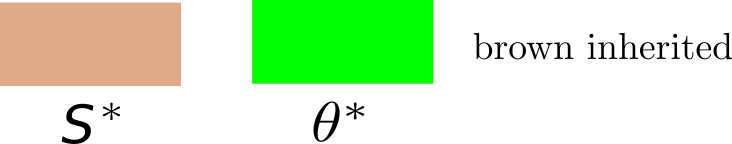
\includegraphics[width=2.5in]
{transfer/fine-tune-params.png}
\end{figure}


\item {\bf Replace final layers of $\cals$
and of $\theta$ by new ones}.
$\cals^*=\cals$ and 
$\theta^*=\theta$ except for final  layers,

For example, in an ANN,
replace the final layers by new ones,
and use $\cald^*$ to 
find the parameters of those
new final layers.

\begin{figure}[h!]
\centering
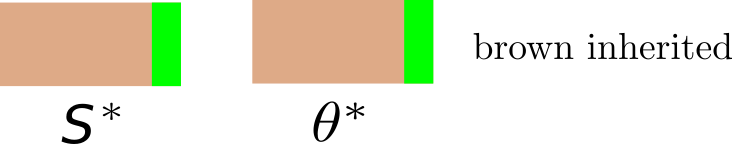
\includegraphics[width=2.5in]
{transfer/last-layer-new.png}
\end{figure}


\item {\bf Transfer only
the  TPM of a single node $\rvy$ of $\calb$}.
$\cals^*$ and $\theta^*$ are new
except $P^*(y|pa(y))=P(y|pa(y))$.

\begin{figure}[h!]
\centering
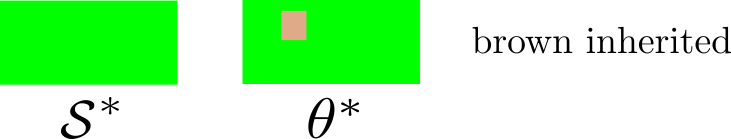
\includegraphics[width=2.5in]
{transfer/one-tpm.png}
\end{figure}

\end{enumerate}







